\newpage
\section{Realisering}
\label{realiseringOgTest}

\subsection{Kretsopkobling}
Oppkoblingen ble gjort som vist i den prinsippielle løsningen i figur \ref{fig:diffamp}, hvor strømkliden ble realisert som i figur \ref{fig:CurrentSource}. Modellene og verdiene som ble brukt vises i tabell \ref{tab:komnpomenter}. 

\begin{figure}[!h]
    \centering
    \begin{minipage}[c]{0.4\textwidth}
        \centering
        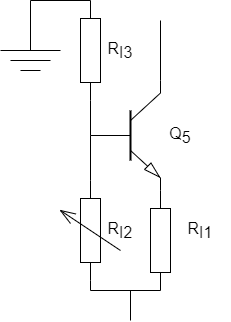
\includegraphics[width=0.6\textwidth]{Bilder/current_source.drawio.png} 
        \caption{Realisert strømkilde.}
        \label{fig:CurrentSource}
    \end{minipage}
    \hfill
    \begin{minipage}[c]{0.5\textwidth}
        \centering
        \begin{tabular}{ |c|c| }
            \hline
            Komponent & Verdi/Produknummer \\ \hline
            \hline
            $Q_1 \& Q_2 \&Q_5$ & BC547A (NPN) \\
            $Q_3 \& Q_4$ & BC557B (PNP) \\
            $R_{I1}$ & $3\text{k}\Omega $ \\
            $R_{I2}$ & $0\Omega - 10\text{k}\Omega$ \\
            $R_{I3}$ & $10\text{k}\Omega$ \\
            \hline
        \end{tabular}
        \\[60pt]
        \caption{Komponenter og verdier brukt i designet.}
        \label{tab:komnpomenter}
    \end{minipage}
\end{figure}

Den oppkoblede kretsen vises i figur \ref{fig:diffamp_realisert}.

\begin{figure}[!h]
    \centering
    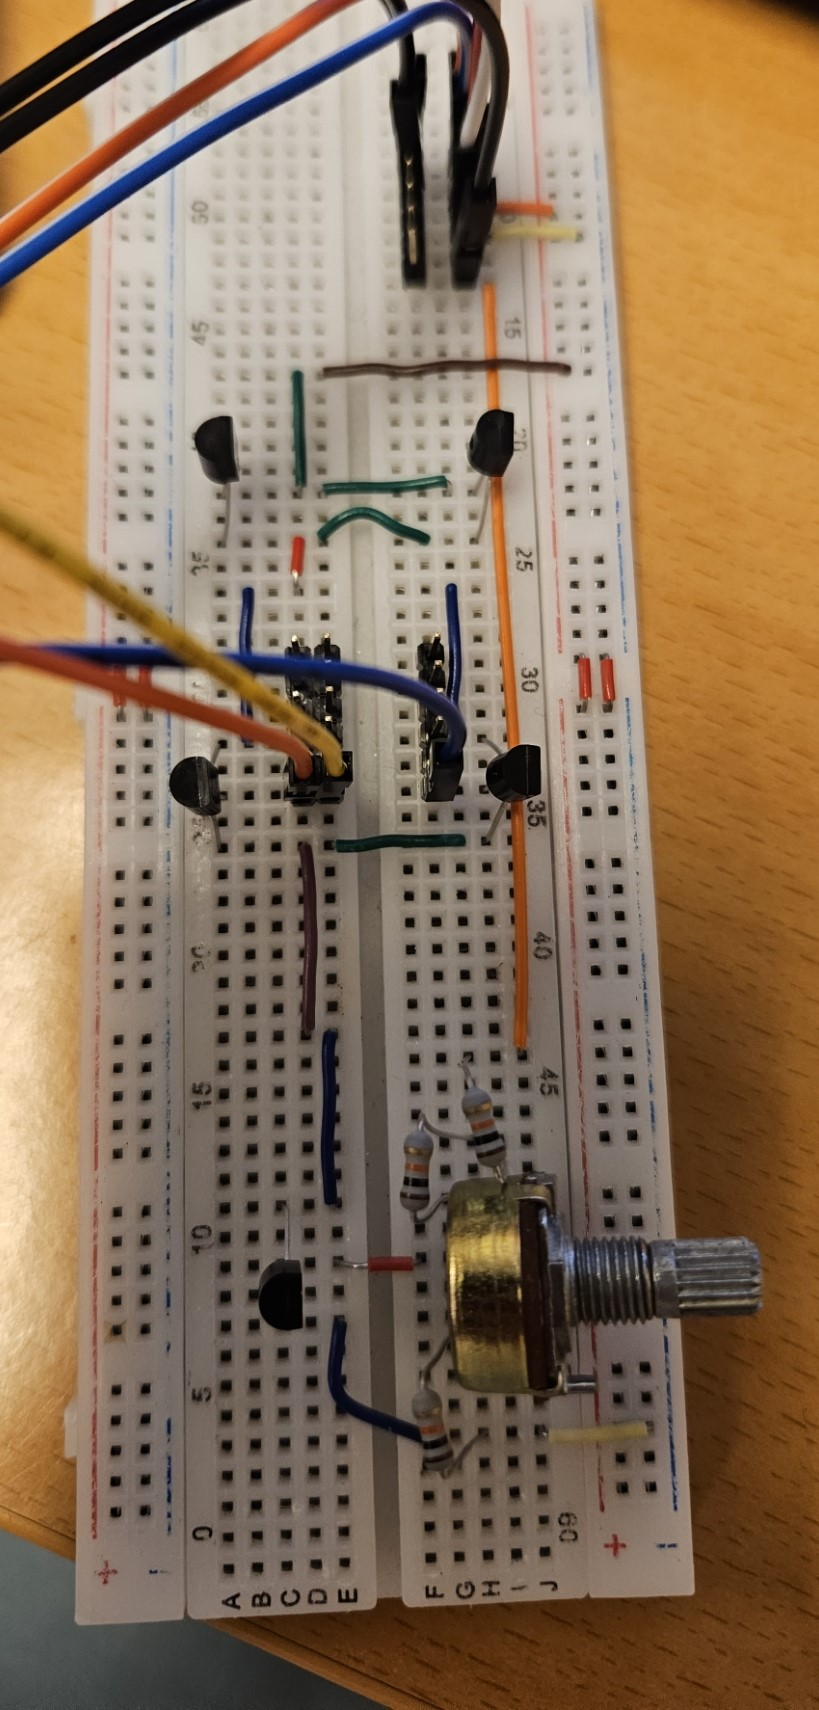
\includegraphics[width=0.4\textwidth, angle=90]{Bilder/feilBilde.jpg}
    \caption{Realisert opperasjonsforsterker}
    \label{fig:diffamp_realisert}
\end{figure}

\clearpage
\subsection{Målinger}
Set ble gjort målinger med ocilioskop og spektrumsanalysator, derretter ble målingene prosesert i python for å finne THD og forsterkning. Målingene ble gjort med en inngangsamplitude på 0.04V og en frekvens på 1kHz. Resultatene av målingene vises i tabell \ref{tab:THD_and_Amplitude_Data}. Ut av tabellen kan vi se at forsterkningen varierer mye når vi ikke har tilbakekobling på utgangen. Vi ser også at når vi setter på en lav lastmotstand så synker forsterkningen kraftig, dette er fordi kretsen ikke klarer å levere den strømmen som kreves. Spektrumsanalysen av utgagnssignalet med last på $R_L = 100k\Omega$ både med og uten tilbakekobling vises i figur \ref{fig:Spectrum_OPAMP_1_tilbake_100KOhm} og i figur \ref{fig:Spectrum_OPAMP_1_100KOhm}. 
%Vi ser at THD er mye lavere med tilbakekobling enn uten. Dette er fordi tilbakekoblingen reduserer forsterkningen, og dermed reduseres også forsterkningen av harmoniske signaler.

\begin{table}[h!]
    \centering
    \begin{tabular}{ |c|c|c|c|c| }
        \hline
        Konfigurasjon & Amplitude inn & Amplitude ut & Forsterkning &THD\\
        \hline
        $R_L = 0$ & 0.04V & 0.90V & 20 &17.92\% \\
        $R_L = 100k\Omega$ & 0.04 & 0.99V & 22& 3.56\% \\
        $R_L = 100\Omega$ & 0.04V & 0.72V & 16& 3.93\% \\
        \hline
        Tilbakekobling $R_L =0$& 0.04V & 0.42V & 9.7& 8.15\% \\
        Tilbakekobling $R_L =100k\Omega$ & 0.04V & 0.42V & 9.4& 8.61\% \\
        Tilbakekobling $R_L =100\Omega$ & 0.04V & 0.21V & 4.7& 9.99\% \\
        \hline
    \end{tabular}
    \caption{THD and Amplitude Data}
    \label{tab:THD_and_Amplitude_Data}
  \end{table}

\begin{figure}[!h]
    \begin{minipage}[c]{0.5\textwidth}
        \centering
        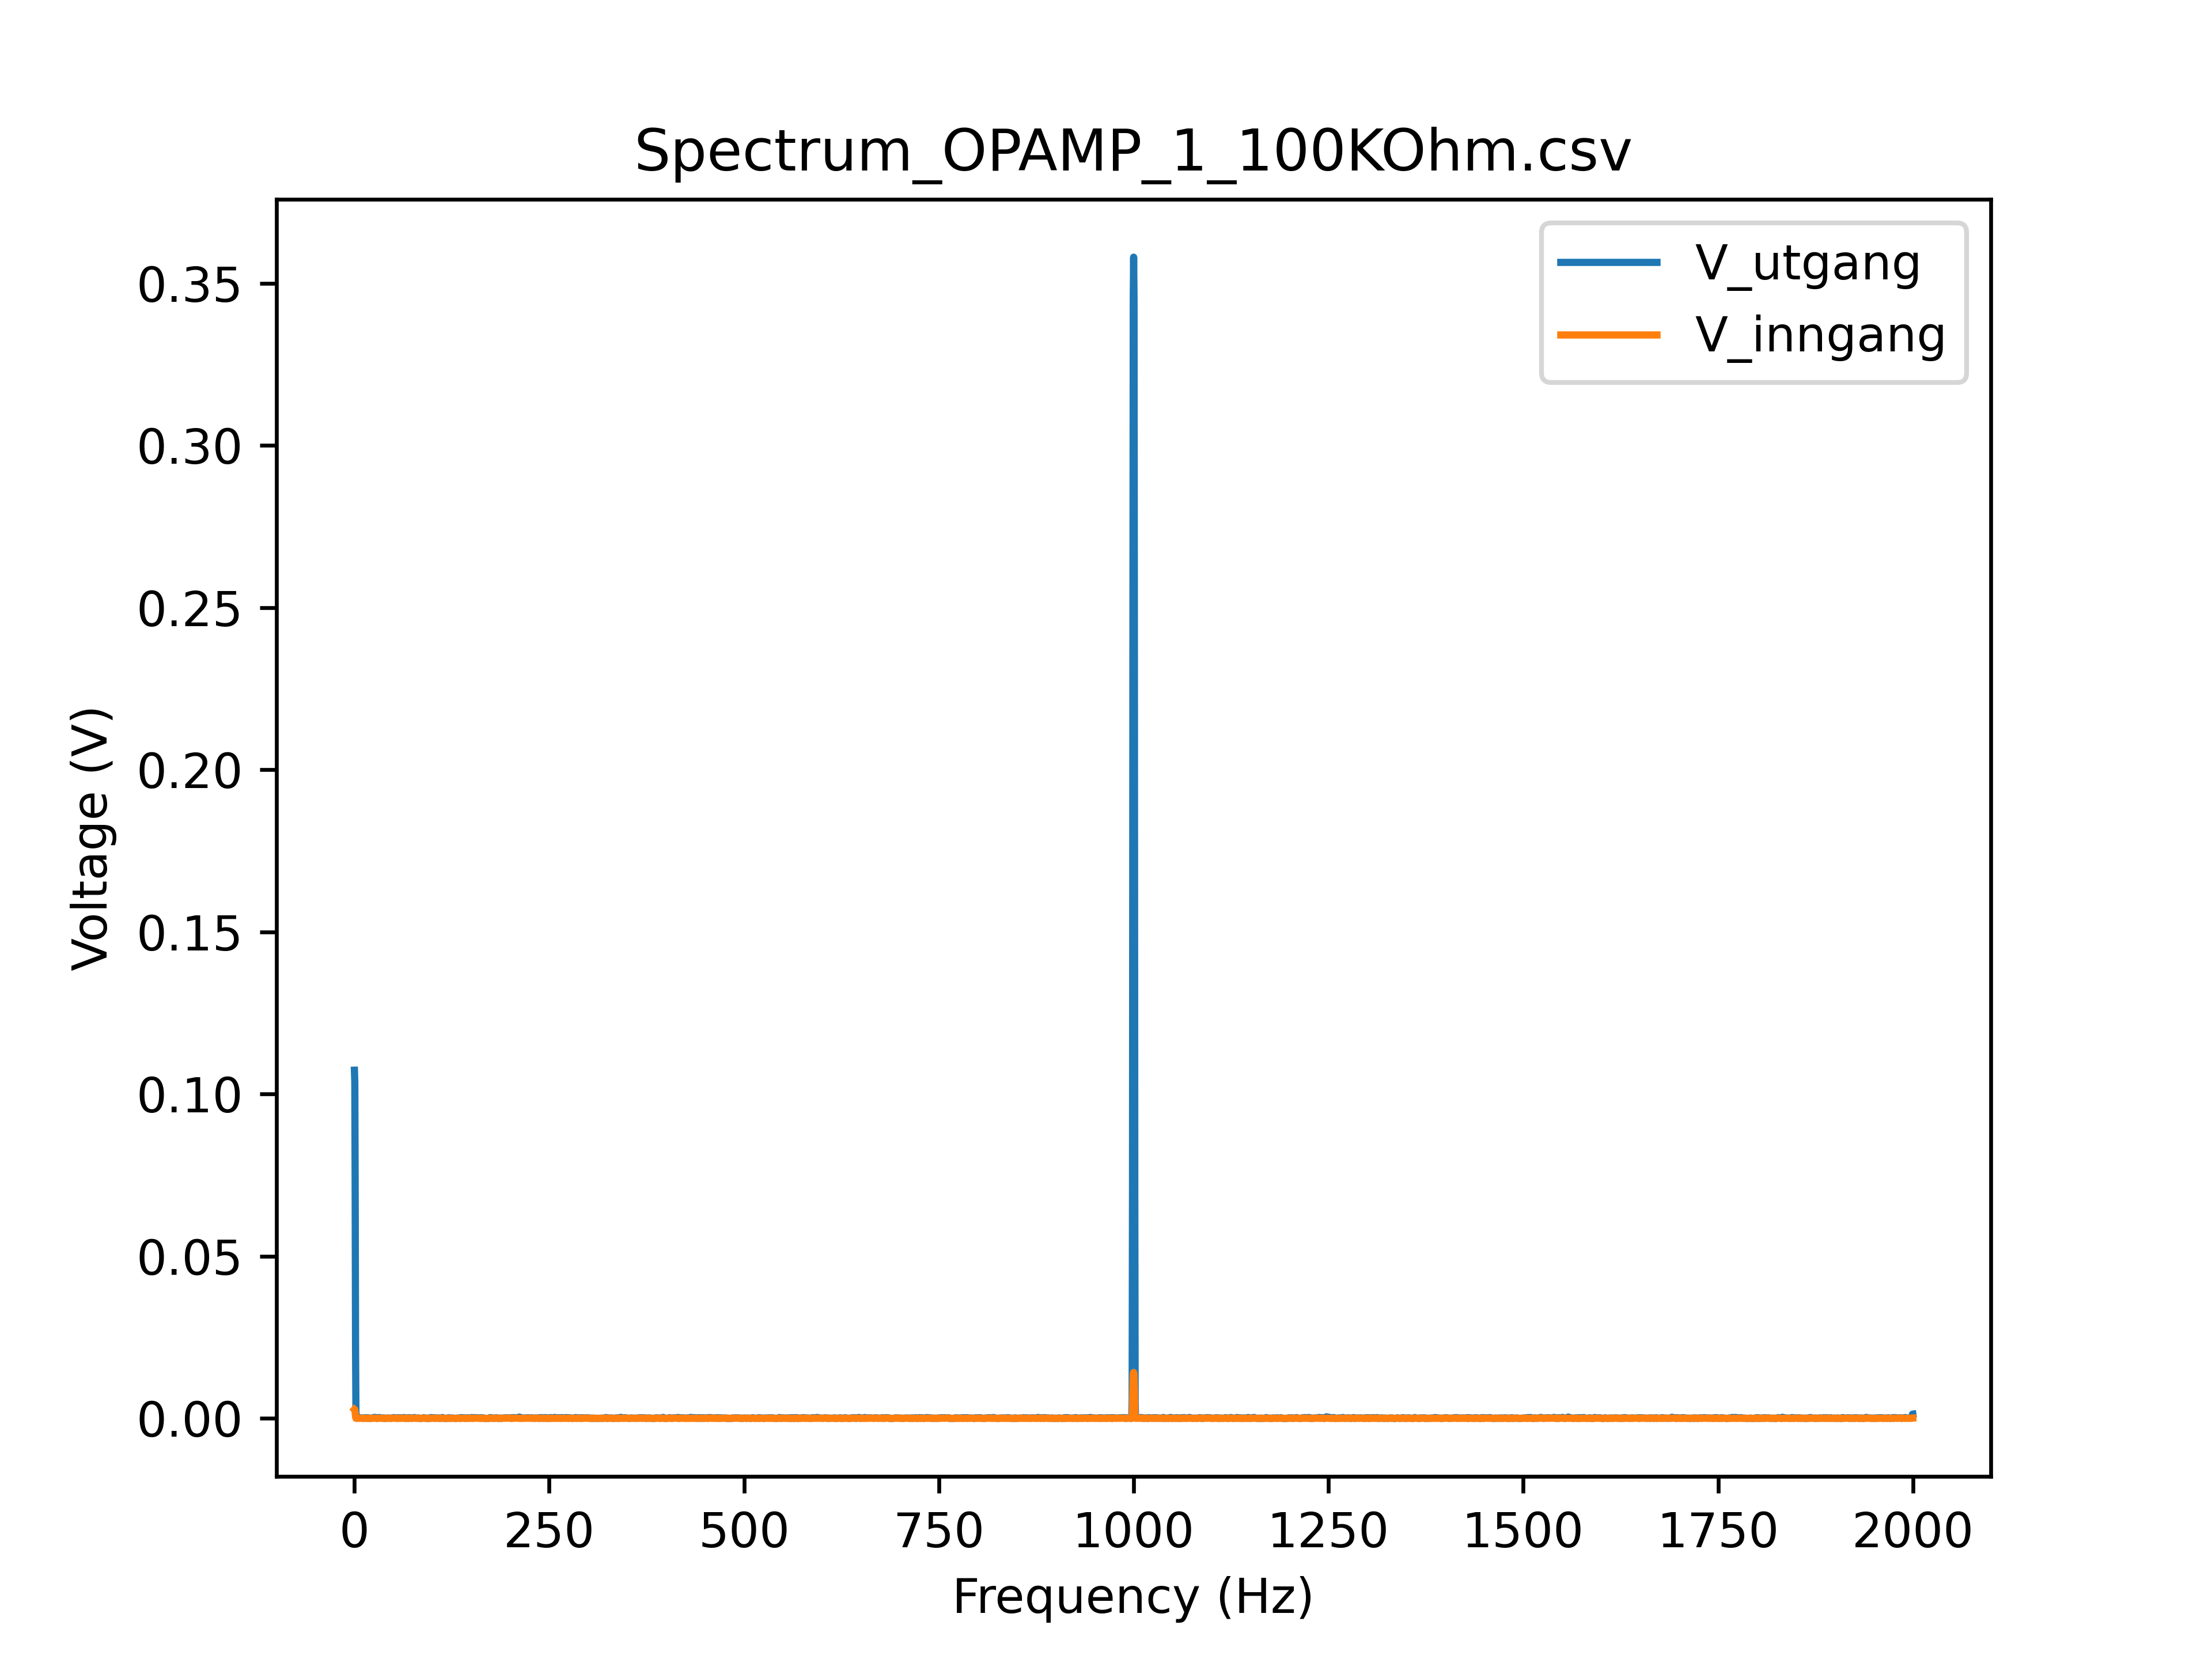
\includegraphics[width=1\textwidth]{Bilder/Spectrum_OPAMP_1_100KOhm.png}
        \caption{Spectrum med $R_L = 100k\Omega$\\ åpen løkke}
        \label{fig:Spectrum_OPAMP_1_100KOhm}
    \end{minipage}
    \hfill
    \begin{minipage}[c]{0.5\textwidth}
        \centering
        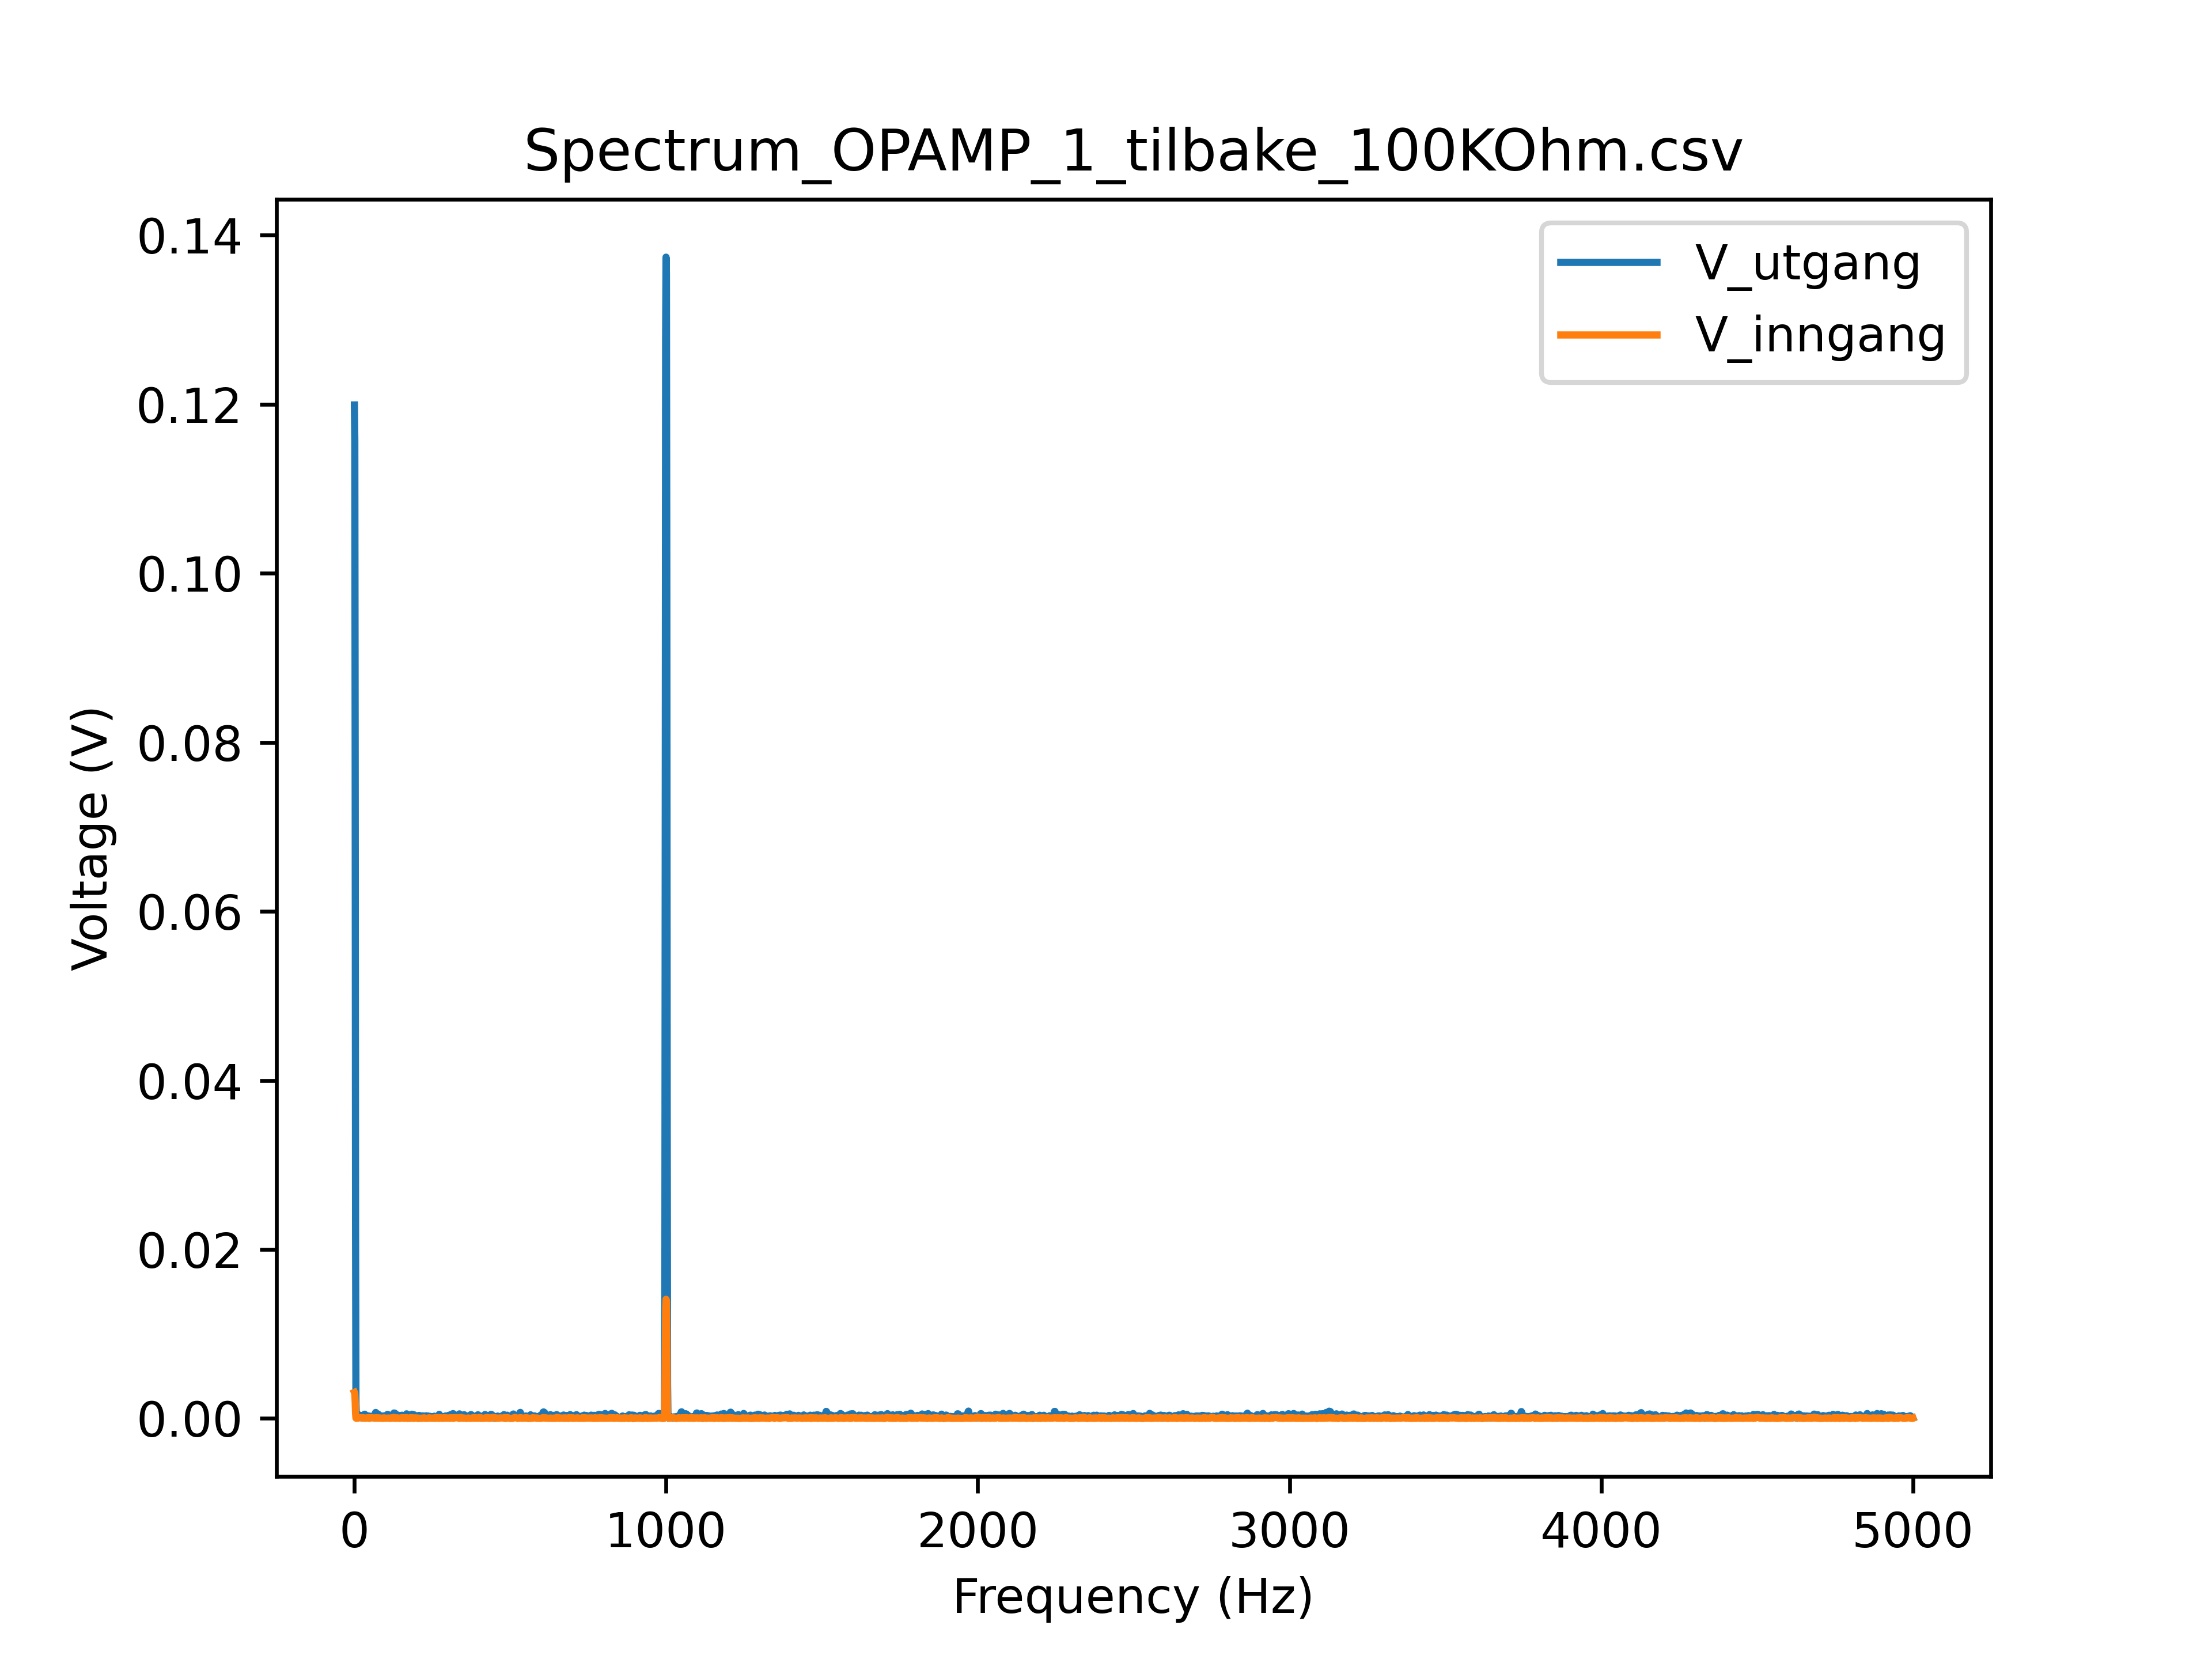
\includegraphics[width=1\textwidth]{Bilder/Spectrum_OPAMP_1_tilbake_100KOhm.png}
        \caption{Spectrum med $R_L = 100k\Omega$\\ tilbakekobling}
        \label{fig:Spectrum_OPAMP_1_tilbake_100KOhm}
    \end{minipage}
\end{figure}

Som vi ser i figur \ref{fig:Spectrum_OPAMP_1_tilbake_100KOhm} så er det mye distorsjon ved 0Hz. Dette er fordi vi har en DC offset på utgangen. Dette kan vi fjerne ved å sette inn en kondensator i tilbakekoblingen. 

\subsection{Forbedringer}
\label{forbedringer}
Denne kretsen kunne blitt bedre hadde man koblet opp en emitter følger ved utgangen.

